\section[Deskriptiv]{Deskriptive Statistik}

\begin{frame}
  {Übersicht}
  \begin{itemize}[<+->]
    \item deskriptive Statistik als Datenaggregation
    \item Verteilungen in Stichproben und Grundgesamtheiten:
      \begin{itemize}
	\item Zentralmaße
	\item Streuung (Varianz)
      \end{itemize}
    \item Beziehungen zwischen ko-variierenden Messungen
    \item Genauigkeiten von Schätzungen quantifizieren (Konfidenzintervalle)
  \end{itemize}
\end{frame}

\begin{frame}
  {Literatur}
  \begin{itemize}
    \item \citet{GravetterWallnau2007}\\
      Achtung! Vermittelt eine falsche Philosophie!\\
      Nur für die Mathematik benutzen.
    \item \citet{Bortz2010}
  \end{itemize}
\end{frame}

\subsection{Motivation}

\begin{frame}
  {Zweck der deskriptiven Statistik}
  \begin{itemize}[<+->]
    \item Mit unbewaffnetem Auge auf Datenmengen zu blicken, ist meistens sinnlos.
    \item In großen Zahlenkolonnen sehen Menschen\\
      nur schlecht Tendenzen und Zusammanhänge.
    \item Um dies zu erleichtern, gruppieren und visualisieren wir die Daten.
  \end{itemize}
\end{frame}


\begin{frame}
  {Grundlegende Kenndaten, die man berichtet}
  \begin{itemize}[<+->]
    \item Definition und (geschätzte) Größe der Grundgesamtheit.\\
    (z.\,B.\ alle lebenden deutschen Erwachsenen)
    \item Stichprobengröße ($N$)
    \item Stichprobenmethode
      \begin{itemize}[<+->]
	\item Zufallsstichprobe (größere Stichprobe)
	\item proportional stratifizierte Stichprobe (Quotenstichprobe)
      \end{itemize}
  \end{itemize}
\end{frame}


\subsection{Skalenniveau}

\begin{frame}
  {Messvariablen und Skalenniveaus}
  Variablen sind folgendermaßen \alert{skaliert}:
  \begin{itemize}[<+->]
    \item \alert{dichotom} (binär) = zwei Kategorien:\\
      männlich, weiblich ; Präteritum, Perfekt
    \item \alert{nominal} (kategorial) = disjunkte Kategorien ohne numerische Interpretation:\\
      Parteizugehörigkeit ; NP, AP, VP
    \item \alert{ordinal} = disjunkte Kategorien, nach Rang geordnet:\\
      Schulnoten ; 5-point oder 7-point scales (Likert scales)\\
    \item \alert{intervall\textasciitilde} = geordnete Werte mit definierten Abständen,\\
      aber mit arbiträrem Nullpunkt: Celsius
    \item \alert{verhältnis\textasciitilde} = wie intervall-,\\
      aber der Nullpunkt ist ein echter Nullpunkt: Kelvin
  \end{itemize}
\end{frame}

\begin{frame}
  {Intervalle vs.\ Verhältnisse}
  \begin{itemize}[<+->]
    \item Wir messen die Größe von Menschen in cm auf einer Verhältnisskala.
      \begin{itemize}[<+->]
	\item 200cm sind das doppelte von 100cm.
	\item Niemand kann kleiner sein als 0cm. 
      \end{itemize}
      \vspace{0.5cm}
    \item Dieselbe Messung als \alert{Abweichung vom Mittel} ergibt eine Intervallskala.
      \begin{itemize}[<+->]
	\item Wer 3 cm größer ist als der Durchschnitt ist doppelt soviel größer\\
	  wie jemand, der 1.5 cm größer ist.
	\item Die erste Person ist aber nicht doppelt so groß wie die zweite.
	\item Außerdem kann man z.B. -3 cm vom Durchschnitt abweichen.
      \end{itemize}
  \end{itemize}
\end{frame}

\begin{frame}
  {Relevanz der Skalenniveaus}
  \begin{itemize}[<+->]
    \item Das SN bestimmt die \alert{zulässigen mathematischen Operationen}\\
      (z.B. Rechenarten).
    \item Also kommen je nach SN nur bestimmte \alert{deskriptive Statistiken} in Frage.
    \item Das gleiche gilt für die Zulässigkeit bestimmter \alert{inferenzstatistischer Tests}\\
      je nach Skalenniveau.
  \end{itemize}
\end{frame}


\subsection{Zentraltendenz}

\begin{frame}
  {Zentraltendenz I}
  Der \alert{Modus} ist der \alert{häufigste Wert} in einer Grundgesamtheit oder Stichprobe.\\
  \alert{Geht bei jedem Skalenniveau.}
  \vspace{-2cm}
  \begin{center}
    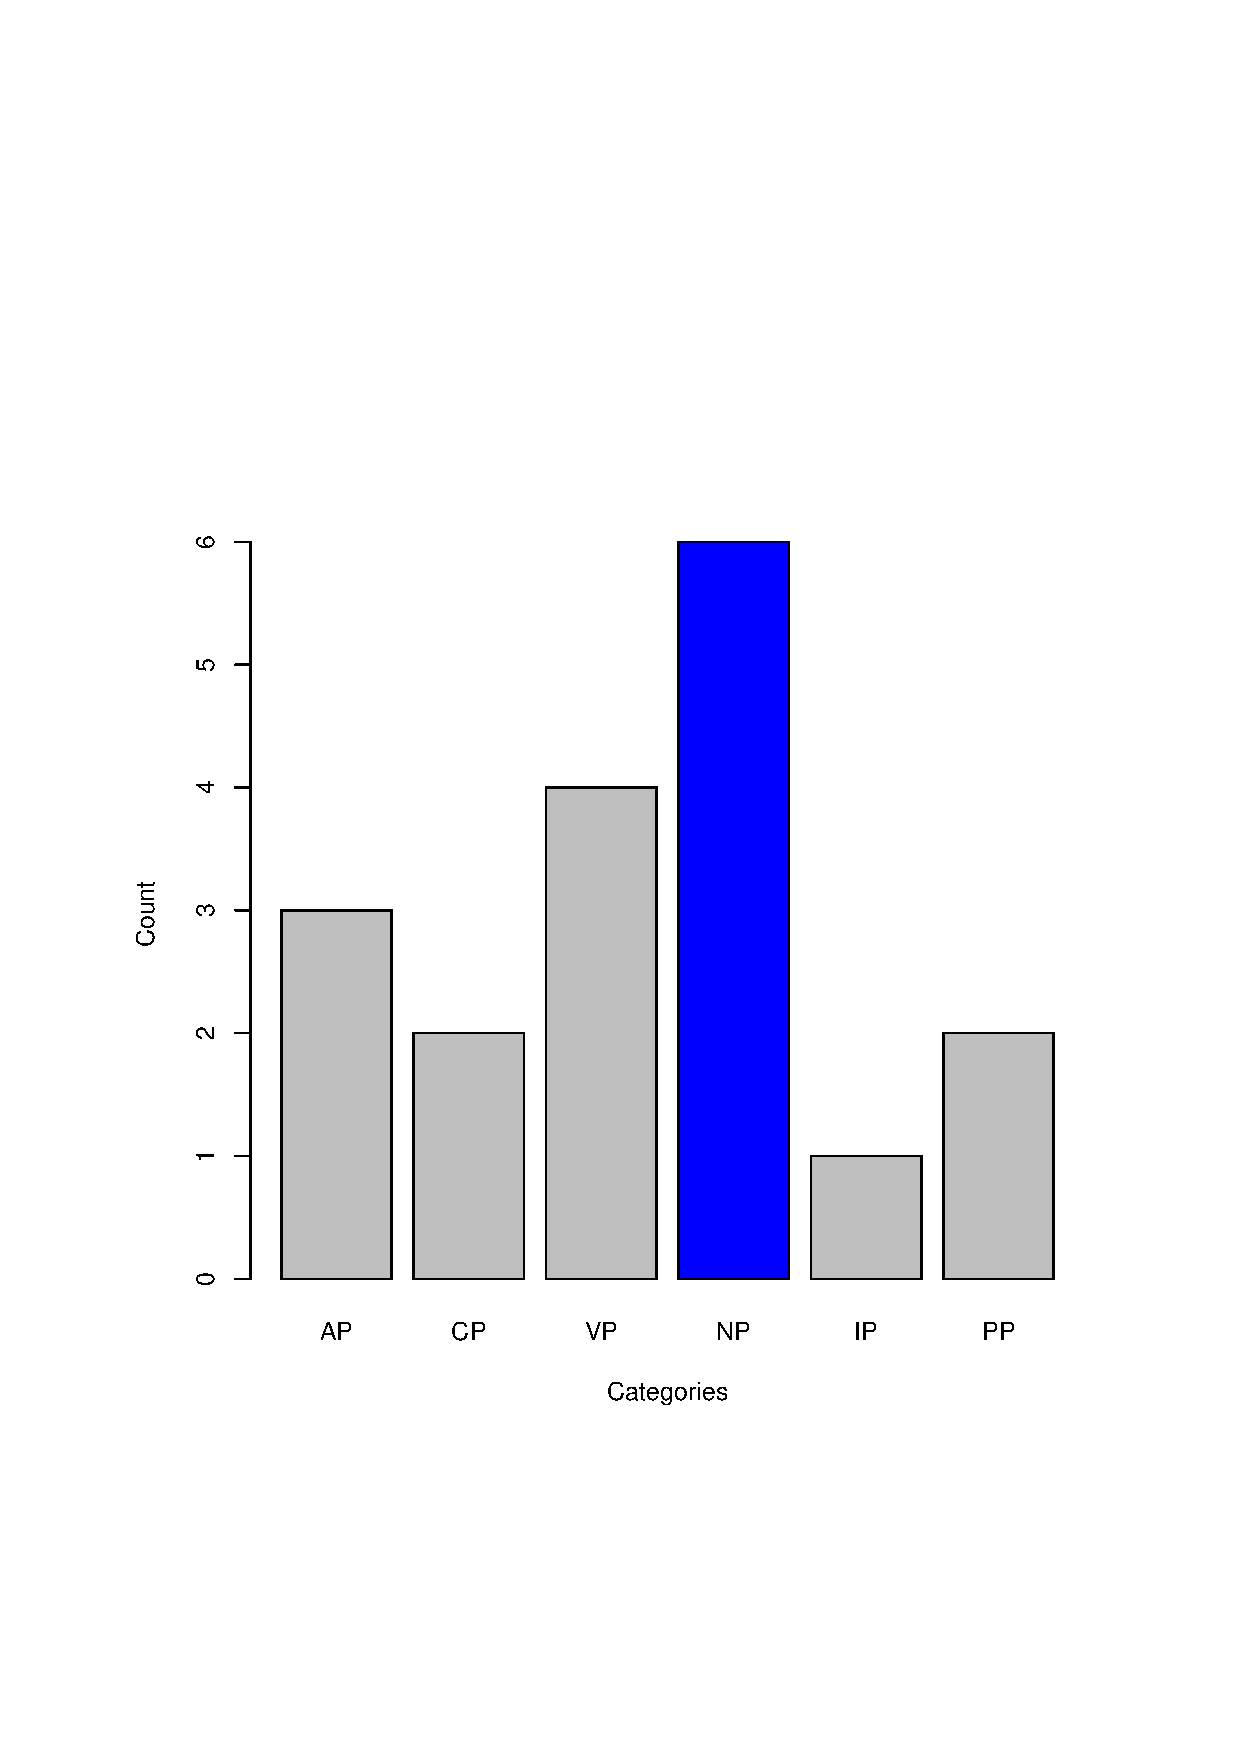
\includegraphics[width=0.5\textwidth]{graphics/mode}
  \end{center}
\end{frame}

\begin{frame}
  {Zentraltendenz II}
  Der \alert{Median} ist der Wert \alert{über und unter dem gleichviele Werte} liegen. \alert{Ordinalskala oder höher.}
  \vspace{-2cm}
  \begin{center}
    \includegraphics[width=0.5\textwidth]{graphics/median}
  \end{center}
\end{frame}

\begin{frame}
  {Zentraltendenz III}
  Das \alert{arithmetische Mittel} $\bar{x}$ ist die Summe aller Werte $x$\\
  dividiert durch Stichprobengröße $n$.\\
  \alert{Intervallskala oder höher.}
  \vspace{-2cm}
  \begin{center}
    \begin{tabular}[!h]{cc}
      \vspace{1.5cm} & \multirow{3}{*}{\includegraphics[width=0.5\textwidth,angle=90]{graphics/mean}} \\
      $\bar{x}=\frac{\sum\limits_{i=1}^{n}x_i}{n}$ \hspace{1.5cm} &  \\
      \vspace{1.5cm} & \\
    \end{tabular}
  \end{center}
\end{frame}

\begin{frame}
  {Zentraltendenz IV}
  Kontinuierliche Variablen und ihr arithmetisches Mittel lassen sich in \alert{Dichteplots} gut visualisieren (per Software).
    \vspace{-2cm}
  \begin{center}
    \includegraphics[width=0.7\textwidth,angle=90]{graphics/meandens}
  \end{center}
\end{frame}


\subsection{Dispersionsmaße}

\begin{frame}
  {Warum sind Dispersionsmaße wichtig?}
  \begin{enumerate}[<+->]
    \item Das Wissen um die Zentraltendenz ist wichtig\\
      als grobe allgemeine Information über die Population.
    \item Aber dieselbe Zentraltendenz kann\\
      das Ergebnis ganz verschiedener Werte sein.
    \item Die Verteilung kann flach, chaotisch, glockenförmig usw. sein.
  \end{enumerate}
\end{frame}

\begin{frame}
  {Verteilungsformen}
  Histogramme von vier Stichproben\\
  mit $\bar{x}=4.389$ und $n=18$.
  \vspace{-0.5cm}
  \begin{center}
    \includegraphics[width=0.5\textwidth]{graphics/fourdists}
  \end{center}
\end{frame}

\begin{frame}
  {Quartile}
  Quartile sind die Punkte, unterhalb derer 25\%, 50\%, 75\% und 100\% (Maximum)\\
  der Werte liegen. Dazu gibt es noch das Minimum (niedrigster Wert).
  \vspace{-0.5cm}
  \begin{center}
    \includegraphics[width=0.5\textwidth]{graphics/fourquartile}
  \end{center}
\end{frame}


\begin{frame}
  {Quartile und Inter-Quartil-Bereich}
  \alert{$IQR = Q_3-Q_1$}\\
  oder ganz einfach: die mittleren 50\%\\
  \begin{center}
    \includegraphics[width=0.5\textwidth]{graphics/boxplotpdf}\\
    {\tiny Attribution: Jhguch (\url{http://en.wikipedia.org/wiki/User:Jhguch}) at en.wikipedia}
  \end{center}
\end{frame}


\begin{frame}
  {Boxplots als bessere Zusammenfassung}
  Boxplots zeigen Median (Linie in der Mitte), oberes und unteres Quartil (Boxen),\\
  1,5-fachen Interquartilabstand zu diesen (gestrichelte Hebel) und Ausreißer (Punkte).
  \vspace{-0.5cm}
  \begin{center}
    \includegraphics[width=0.5\textwidth]{graphics/fourbox}
  \end{center}
\end{frame}


\begin{frame}
  {Varianz und Standardabweichung}
    Die \alert{Varianz $s^2$} ist die quadrierte mittlere Abweichung vom Mittel:\\
      \begin{center}
	\alert{$s^2(x)=\frac{ \sum\limits_{i=1}^{n}(x_i-\bar{x})^2}{n-1}$}
      \end{center}
\pause
      \vspace{0.5cm}
    Die \alert{Standardabweichung $s$} ist die Quadratwurzel der Varianz:\\
      \begin{center}
	\alert{$s(x)=\sqrt{s^2(x)}$}
      \end{center}
      \vspace{0.5cm}

  \pause
    Der Zählerterm der Varianz heißt auch \alert{Summe der Quadrate}:\\
  \begin{center}
    $SQ(x)=\sum\limits_{i=1}^{n}(x_i-\bar{x})^2$
  \end{center}
\end{frame}

\begin{frame}
  {Unterschiedliche Stabw}
  Die erste Stichprobe hat $s=1.91$,\\
  die zweite $s=3.01$ (beide $\bar{x}=4.389$).
  \vspace{-2cm}
  \begin{center}
    \includegraphics[width=0.7\textwidth,angle=90]{graphics/stdevs}
  \end{center}
\end{frame}

%\begin{frame}
%  {Standardfehler}
%  Der Standardfehler gibt die Güte des Stichprobenmittelwerts\\
%  relativ zum Mittelwert der Grundgesamtheit an.\\
%  \begin{center}
%    \begin{tabular}{cc}
%      \alert{$SF(x)=\frac{s(x)}{\sqrt{n}}$} & \\
%    \end{tabular}
%  \end{center}
%  Man erhält die Standardabweichung der Mittelwerte\\
%  von beliebig vielen gleich großen Stichproben\\
%  vom Mittelwert der Grundgesamtheit.\\[3ex]
%  Dies ist der \alert{SF für Mittelwerte}, später bekommen wir\\
%  den \alert{SF für Anteilswerte}.
%\end{frame}

\begin{frame}
  {z-Wert}
  Um wie viele Standardabweichungen weicht jeder Datenpunkt vom Mittel ab?\\
  Für jeden Punkt: \alert{$z(x_i)=\frac{x_i-\bar{x}}{s(x)}$}\\[3ex]

  Bsp.: $\alert{x}=[3.9, 4.3, 7.2, 8.5, 11.1, 12.1, 14.0, 20.7]$\\[1ex]
  $\alert{\bar{x}}=$\onslide<2->{$10.225$}\\[1ex]
  \onslide<3->{$\alert{s^2(x)}=$}\onslide<4->{$\frac{(3.9-10.255)^2+\ldots+(20.7-10.225)^2}{8-1}=$}\onslide<5->{$\frac{215.495}{7}=$}\onslide<6->{$30.785$}\\[1ex]
  \onslide<7->{$\alert{s(x)}=$}\onslide<8->{$\sqrt{30.785}=$}\onslide<9->{$5.548$}\\[1ex]
  \onslide<10->\onslide<11->{$\alert{z}=[\frac{3.9-10.225}{5.548}$, \ldots, $\frac{20.7-10.225}{5.548}]=$}\\[1ex]
  \onslide<12->{\ \,\ \ \ \ $[-1.140, -1.068, -0.545, -0.311, 0.158, 0.338, 0.680, 1.888]$}
\end{frame}

\subsection{Bivariate Statistiken}

\begin{frame}
  {Zähldaten von zwei Variablen}
  Zähldaten von zwei Variabeln (egal wieviel Ausprägungen)\\
  sind ideal als \alert{Kreuztabelle} darstellbar.\\
  \vspace{1cm}

  \begin{center}
    \begin{tabular}{|c|c|c|}
      \cline{2-3}
      \multicolumn{1}{c|}{} & \textbf{Variable 1: Wert 1} & \textbf{Variable 1: Wert2} \\
      \hline
      \textbf{Variable 2: Wert 1} & Anzahl $x_{11}$ & Anzahl $x_{12}$ \\
      \textbf{Variable 2: Wert 2} & Anzahl $x_{21}$ & Anzahl $x_{22}$ \\
      \hline
    \end{tabular}
  \end{center}
\end{frame}

\begin{frame}
  {Korrelationen}
  Korrelationskoeffizienten helfen, den Zusammenhang zwischen Variablen,\\
  die mindestens ordinalskaliert sind, numerisch zu erfassen.\\
  Z.\,B. die hier geplotteten $x$ und $y$:
  \vspace{-0.5cm}
  \begin{center}
    \includegraphics[width=0.4\textwidth]{graphics/corrplot}
  \end{center}
\end{frame}


\begin{frame}
  {Kovarianz}
  Die Kovarianz kombiniert die Maße, zu denen die \alert{zwei Messwerte} pro Datenpunkt\\
  vom \alert{jeweiligen Mittel der Messwertreihen} abweichen.\\
  \begin{center}
    \alert{$cov(x,y)=\frac{\sum\limits_{i=1}^{n}(x_i-\bar{x})\cdot(y_i-\bar{y})}{n-1}$}\\
  \end{center}
  \pause
  Sind $x_i-\bar{x}$ und $y_i-\bar{y}$ positiv oder negativ, ist der Beitrag ihres Produkts\\
  zur Kovarianz positiv, bei ungleichen Vorzeichen negativ.
  \pause
  \begin{center}
    Der Zählerterm heißt auch \alert{Summe der Produkte}:\\
    $SP(x,y)=\sum\limits_{i=1}^{n}(x_i-\bar{x})\cdot(y_i-\bar{y})$
  \end{center}
\end{frame}


\begin{frame}
  {Kovarianz: Illustration 1}
  Zwei Messvariablen (Vektoren): $x$ und $y$
  \begin{center}
    \includegraphics[width=0.4\textwidth]{graphics/cov01}
  \end{center}
\end{frame}


\begin{frame}
  {Kovarianz: Illustration 2}
  Koordinate von $\langle\bar{x},\bar{y}\rangle$
  \begin{center}
    \includegraphics[width=0.4\textwidth]{graphics/cov02}
  \end{center}
\end{frame}


\begin{frame}
  {Kovarianz: Illustration 3}
  Punktvarianzen: $x_3-\bar{x}=-7.81$ und $y_3-\bar{y}=-5.80$\\
  \alert{$-7.81\cdot-5.80=45.30$}
  \begin{center}
    \includegraphics[width=0.4\textwidth]{graphics/cov03}
  \end{center}
\end{frame}


\begin{frame}
  {Kovarianz: Illustration 4}
  Punktvarianzen: $x_{17}-\bar{x}=4.95$ und $y_{17}-\bar{y}=7.11$\\
  \alert{$4.95\cdot7.11=35.19$}
  \begin{center}
    \includegraphics[width=0.4\textwidth]{graphics/cov04}
  \end{center}
\end{frame}


\begin{frame}
  {Kovarianz: Illustration 5}
  Puntvarianzen für alle $\langle x_i,y_i\rangle$\\
  $cov(x,y)=34.52$
  \begin{center}
    \includegraphics[width=0.4\textwidth]{graphics/cov05}
  \end{center}
\end{frame}


\begin{frame}
  {Kovarianz: Illustration 6}
  "`Ausreißer"' bei -- im Prinzip -- positiver Kovarianz:\\
  \alert{Negatives Produkt} der Punktvarianzen
  \begin{center}
    \includegraphics[width=0.4\textwidth]{graphics/cov06}
  \end{center}
\end{frame}


\begin{frame}
  {Kovarianz: Illustration 7}
  Punktvarianzen: $x_{21}-\bar{x}=6.77$ und $y_{21}-\bar{y}=-8.79$\\
  \alert{$6.77\cdot-8.79=-59.51$}
  \begin{center}
    \includegraphics[width=0.4\textwidth]{graphics/cov07}
  \end{center}
\end{frame}

\begin{frame}
  {Kovarianz: Negative Kovarianz}
  Wenn die Abhängigkeit zwischen den Werten tendentiell negativ ist,\\
  sind die Produkte der Punktvarianzen überwiegend negativ.\\
  $cov(x,y)=-33.77$
  \begin{center}
    \includegraphics[width=0.4\textwidth]{graphics/cov08}
  \end{center}
\end{frame}

\begin{frame}
  {Kovarianz: Null annähernd}
  Wenn es keine besondere Abhängigkeit gibt,\\
  nähert sich die Kovarianz 0:\\
  $cov(x,y)=-1.74$\\
  \vspace{-1cm}
  \begin{center}
    \includegraphics[width=0.4\textwidth]{graphics/cov09}
  \end{center}
\end{frame}

\begin{frame}
  {Kovarianz zu Korrelationskoeffizient $r$}
  Während die Kovarianz \alert{von der Größe der Werte} abhängt,\\
  macht der Korrelationskoeffizient Kovarianzen vergleichbar:\\[3ex]

  \begin{center}
    $r(x,y)=\frac{cov(x,y)}{s(x)\cdot s(y)}$
  \end{center}
  \vspace{0.5cm}
  \pause
  Dies ist die \alert{Pearson-Korrelation}, später kommen noch andere Korrelationen.
\end{frame}


\subsection{Konfidenzintervalle}



\begin{frame}
  {Anteilswerte, Beispiel}
  \begin{itemize}[<+->]
    \item Das Verb \textit{essen} kommt manchmal mit, manchmal\\
      ohne Akkusativ (direktes Objekt) vor.
    \item \alert{mit dO 39, ohne dO 61}.
    \item Wenn wir in dieser Situation Stichproben mit \alert{n=100} ziehen, werden wir nicht immer genau diese Werte messen, sondern sie zwar häufig gut approximieren, manchmal aber auch stark abweichende Anteilswerte messen.
    \item In welchem Bereich liegen 95\% aller Messwerte bei n=100?
    \item Diese Frage beantwortet das \alert{95\%-Konfidenzintervall}.
    \item Es sagt uns, wie gut Stichproben einer bestimmten Größe bestimmte Anteilswerte approximieren.
  \end{itemize}
\end{frame}

\begin{frame}
  {Argumentation zum KI}
  \begin{itemize}[<+->]
    \item Annahme: Wahrer \alert{Anteilswert in der Grungesamtheit} ist $P$.
    \item In \alert{Stichproben der Größe $n$} misst man einen \alert{Stichprobenanteil $p$}.
    \item Die meisten $p$ liegen nah an $P$, sehr wenige weit weg davon.
    \item Wenn man beliebig viele $p$ hat, verteilen sie sich so um $P$,\\
      dass eine Standardabweichung dem \alert{Standardfehler} entspricht.
    \item Der Standardfehler ist der Erwartungswert für die Standardabweichung\\
      sehr vieler Messwerte (um den wahren Wert).
    \item Außerdem weiß man, dass die \alert{$p$ normalverteilt um $P$} sind.\\
      Das folgt für groß genuge Stichproben aus dem \alert{Zentralen Grenzwertsatz}.
    \item Bei einer Normalverteilung weiß man, \alert{wieviel Prozent der Messwerte}\\
      \alert{in einem Bereich $\pm q\cdot s$} (für beliebige $q$) vom Mittel liegen.
  \end{itemize}
\end{frame}

\begin{frame}
  {Erstens: Standardfehler}
  Wir brauchen also für Stichproben der Größe $n$ den SF für den\\
  tatsächlichen Anteilswert $P$.\\[3ex]

  \begin{center}
    $SF(P)=\sqrt{\frac{p\cdot(1-p)}{n}}$\\

    \vspace{1cm}
    Bsp. für $p=0.39$ und $n=100$: $SF(p)=\sqrt{\frac{0.39\cdot(1-0.39)}{100}}=0.0488$
  \end{center}
\end{frame}

\begin{frame}
  {Zum Standardfehler}
  \begin{center}
    \alert{$SF(p)=\sqrt{\frac{p\cdot(1-p)}{n}}$}\\

    \vspace{.1cm}
    Bsp.: $SF(p)=\sqrt{\frac{0.39\cdot(1-0.39)}{100}}=0.0488$
  \end{center}

  \vspace{.2cm}
  \pause
  \begin{itemize}[<+->]
    \item Anders gesagt: Wenn man beliebig viele Stichproben der Größe $n=100$\\
      aus einer Grundgesamtheit zieht, in der der \alert{wahre Anteilswert} $P=0.39$ ist,\\
      ist eine Standardabweichung aller $p$ (also der Standardfehler) $SF=0.0488$.
  \end{itemize}
\end{frame}

\begin{frame}
  {Normalverteilung und z-Wert für Konfidenzniveau}
  \begin{itemize}[<+->]
    \item Um das KI für die gewünschte Konfidenzniveau zu ermitteln,\\
      müssen wir wissen, wie sich Werte um das geschätzte Mittel verteilen.
    \item Schätzverteilung dank Zentralem Grenzwertsatz: \alert{Normalverteilung}
    \item Vorteil: Es ist genau bekannt, wieviel Werte je nach $s$\\
      in einem bestimmten Intervall liegen.
  \end{itemize}
  \pause
  \begin{center}
    \includegraphics[width=0.3\textwidth]{graphics/normal}
  \end{center}
\end{frame}

\begin{frame}
  {Zweitens: z-Wert}
  \begin{itemize}[<+->]
    \item Wir müssen nun wissen, wieviele Standardabweichungen\\
      bei der Normalverteilung $95\%$ der Fläche definieren.
    \item Wenn es \alert{symmetrische $95\%$} werden sollen,\\
      müssen \alert{oben und unten je $2.5\%$} abgetrennt werden.
    \item Dazu gibt es Tabellen oder die\\
      \alert{Quantil-Funktion der Normalverteilung \texttt{qnorm()}} in \texttt{R}.
    \item \texttt{qnorm(0.025, lower.tail=FALSE)} $\Rightarrow 1.959964$
    \item Also: \alert{$z=1.96$}
  \end{itemize}
\end{frame}

\begin{frame}
  {Drittens: Konfidenzintervall}
  \begin{itemize}[<+->]
    \item Da \alert{der Standardfehler genau einer Standardabweichung entspricht},\\
      muss er nun \alert{mit dem z-Wert multipliziert} werden.
  \end{itemize}
  \pause
  \vspace{.5cm}
  \begin{center}
    \alert{$KI=p\pm z\cdot SF(p)$}

    \vspace{.2cm}
    Bsp.: $KI=0.39\pm1.96\cdot 0.0488=0.39\pm0.096=0.29, 0.49$
  \end{center}
\end{frame}

\begin{frame}
  {Interpretation}
  Das \alert{Konfidenzinterval} ist in unserem Fall also\\
  \vspace{.1cm}
  \begin{center}
    \alert{0.29 bis 0.49}  
  \end{center}
  \pause
  \begin{itemize}[<+->]
    \item In 95\% aller Stichproben mit $n=100$ läge der Messwert\\
      beim wahren Anteil von $0.39$ zwischen $0.29$ und $0.49$.
    \item Oft wird auf Basis einer Stichprobe mit der Göße n ein Anteilswert p\\
      geschätzt und dann für diesen das Konfidenzintervall ausgerechnet.
    \item Das kann man zwar machen, aber man lernt dadurch nichts über die GG!
    \item Ggf.\ kann uns das so errechnete KI einen Eindruck davon geben,\\
      wie genau Stichproben der Größe n bei einem Anteil wie dem gemessenen\\
      ungefähr sind.
      \vspace{\baselineskip}
    \item \alert{Der gemessene Anteil p kann aber eine totale Fehlschätzung sein!}
    \item Die Philosophie bezieht sich auf das \alert{wiederholte Berechnen} von KIs.
  \end{itemize}
\end{frame}

\begin{frame}
  {Verboten: Balkendiagramm mit Konfidenzintervall}
  Ein solches Diagramm signalisiert \alert{fälschlicherweise},\\
  dass das Konfidenzintervall uns etwas über die GG sagt!\\
  \vspace{-1cm}
  \begin{center}
    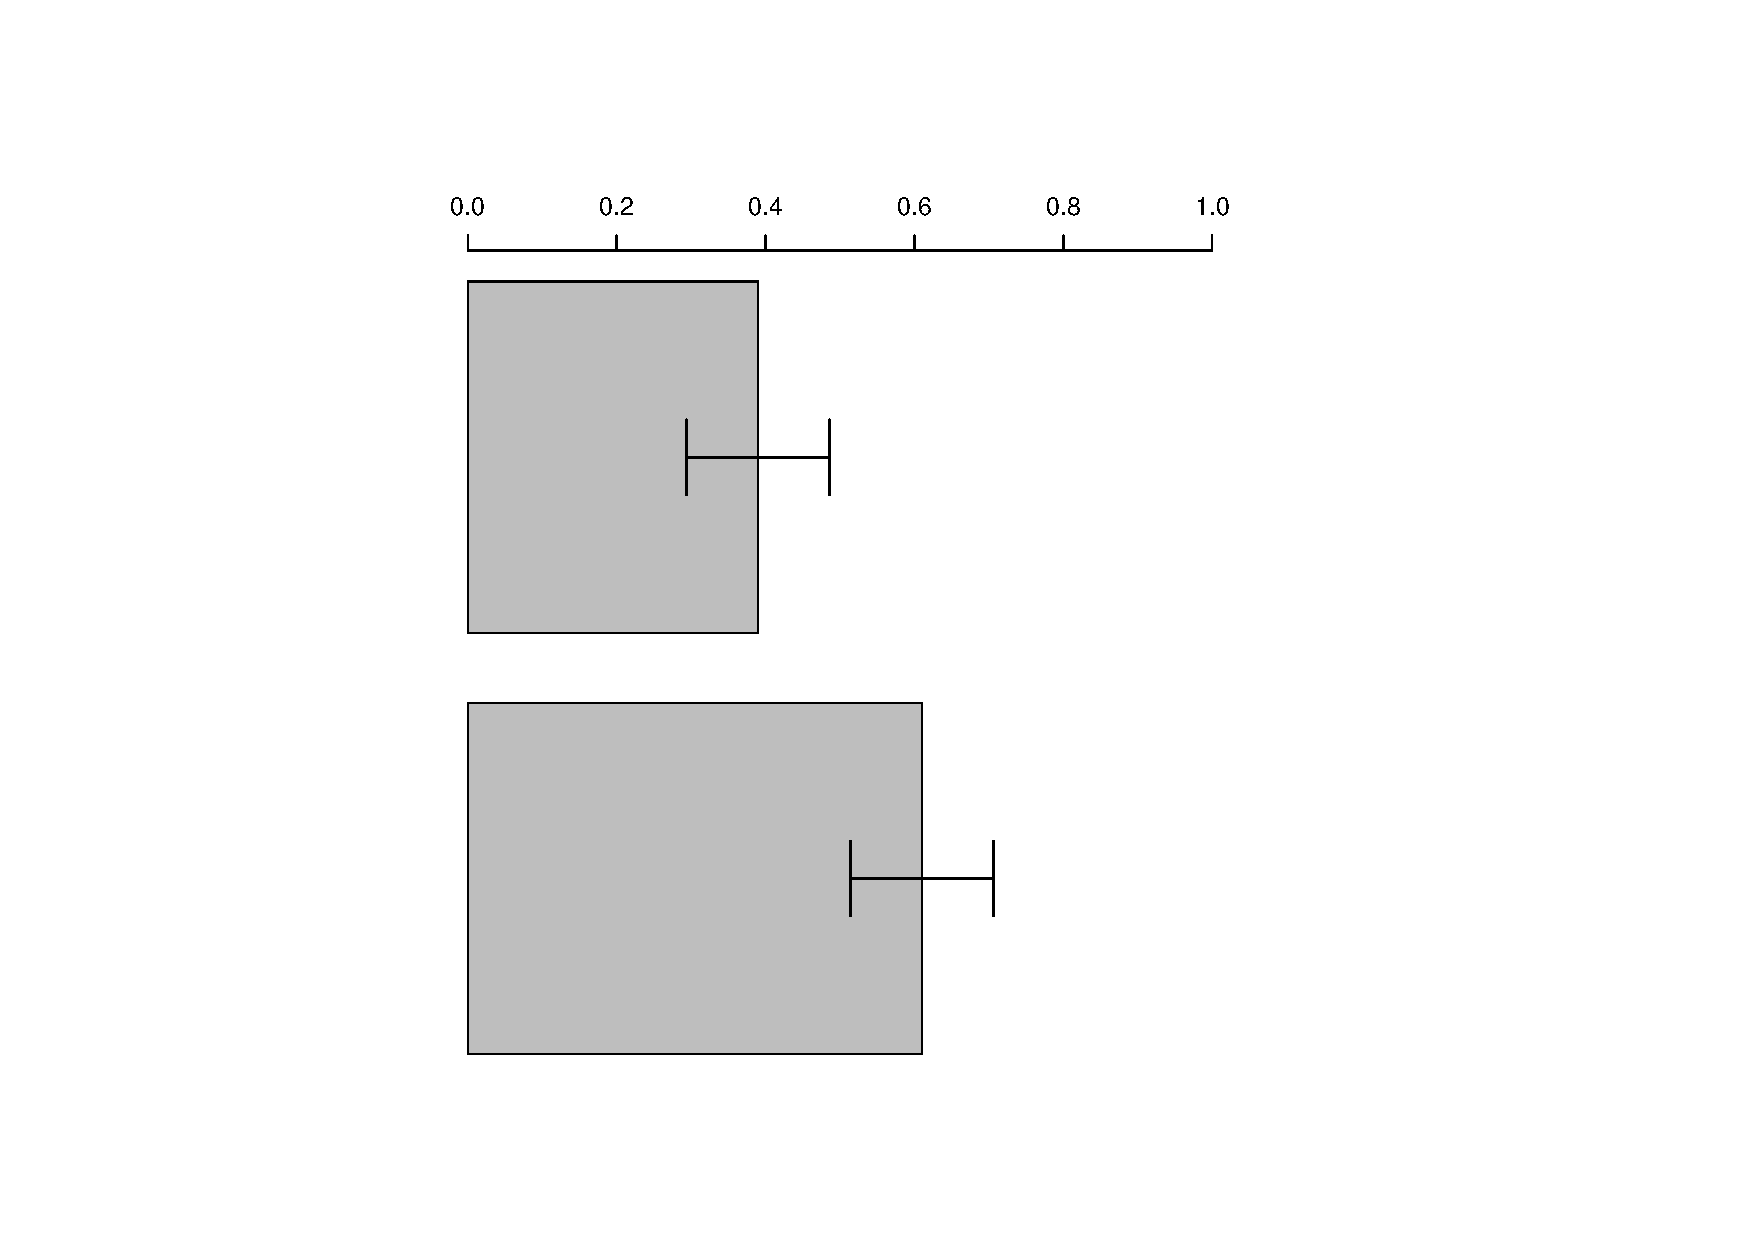
\includegraphics[width=0.7\textwidth,angle=90]{graphics/ki}
  \end{center}
\end{frame}

\ifdefined\TITLE
  \section{Nächste Woche | Überblick}

  \begin{frame}
    {Einzelthemen}
    \begin{enumerate}
      \item Inferenz
      \item Deskriptive Statistik
      \item \alert{Nichtparametrische Verfahren}
      \item z-Test und t-Test
      \item ANOVA
      \item Freiheitsgrade und Effektstärken
      \item Power und Severity
      \item Lineare Modelle
      \item Generalisierte Lineare Modelle
      \item Gemischte Modelle
    \end{enumerate}
  \end{frame}
\fi
